% =====================================================================
%  main.tex
%  Paper: Analysis of Prompt Engineering Techniques and Their
%         Algorithmic Effect on LLM Output
%  Authors: Brishav Joshi, Nitesh Pant, Sarwagya Acharya
%  Final manuscript: Parts 1--3 assembled (Introduction, Related
%  Work, Taxonomy, Framework, Experiments, Results, Discussion,
%  Limitations, Conclusion).
%
%  Skeleton copied verbatim from
%  IEEE-conference-template-062824/IEEE-conference-template-062824.tex.
%  All package choices and class options are pinned by AGENTS.md §4
%  and format.md — do not add new packages.
% =====================================================================

\documentclass[conference]{IEEEtran}
\IEEEoverridecommandlockouts
% The preceding line is only needed to identify funding in the first
% footnote. If that is unneeded, please comment it out.
%Template version as of 6/27/2024

\usepackage{cite}
\usepackage{amsmath,amssymb,amsfonts}
\usepackage{algorithmic}
\usepackage{graphicx}
\usepackage{textcomp}
\usepackage{xcolor}
\usepackage{booktabs}
\usepackage{url}

\def\BibTeX{{\rm B\kern-.05em{\sc i\kern-.025em b}\kern-.08em
    T\kern-.1667em\lower.7ex\hbox{E}\kern-.125emX}}

\begin{document}

% ---------------------------------------------------------------------
%  Title
%  Rules: no sub-title, no symbols, no special characters, no math,
%         no footnotes in title.  See AGENTS.md §4.1 and format.md.
% ---------------------------------------------------------------------
\title{Analysis of Prompt Engineering Techniques and Their Algorithmic
Effect on Large Language Model Output}

% ---------------------------------------------------------------------
%  Authors
%  Order is permanent for citations/indexing.  Affiliation is shared
%  across all three authors.  Email/affiliation lines are placeholders
%  (<<...>>) -- replace before submission.  See AGENTS.md §4.2.
% ---------------------------------------------------------------------
\author{
\IEEEauthorblockN{1\textsuperscript{st} Sarwagya Acharya}
\IEEEauthorblockA{\textit{Department of Electronics and Computer Engineering} \\
                 \textit{National College of Engineering, Tribhuvan University} \\
                 Kathmandu, Nepal \\
                 formalsarwagya@gmail.com}
\and
\IEEEauthorblockN{2\textsuperscript{nd} Nitesh Pant}
\IEEEauthorblockA{\textit{Department of Electronics and Computer Engineering} \\
                 \textit{National College of Engineering, Tribhuvan University} \\
                 Kathmandu, Nepal \\
                 np3234@gmail.com}
\and
\IEEEauthorblockN{3\textsuperscript{rd} Brishav Joshi}
\IEEEauthorblockA{\textit{Department of Electronics and Computer Engineering} \\
                 \textit{National College of Engineering, Tribhuvan University} \\
                 Kathmandu, Nepal \\
                 <<EMAIL\_BRISHAV>>}
}

\maketitle

% ---------------------------------------------------------------------
%  Abstract
%  Final abstract, written after the results (AGENTS.md §2 Part 3
%  rule).  No math, no symbols, no footnotes.  See AGENTS.md §4.3.
% ---------------------------------------------------------------------
\begin{abstract}
Prompt engineering techniques are widely reported to improve the
output of large language models (LLMs), but their measured effects
are rarely separated from the wording of the prompt or from the
decoding configuration used to produce the output.  This paper treats
six prompting techniques---direct answering, zero-shot and few-shot
chain-of-thought (CoT), self-consistency, tree-of-thoughts, and
ReAct---as algorithmic operators on the conditional output
distribution and evaluates them in a controlled factorial study
across three Llama 3.1 models and four tasks.  On grade-school
arithmetic, few-shot CoT raised accuracy from 58.4\% to 83.1\% for the
8B model and from 74.6\% to 94.2\% for the 70B model, gains that
rival or exceed the difference between adjacent model scales.  An
algorithmic effect ratio of 0.78 shows that most of the benefit
survives rewording of the prompt.  Composite techniques were
decomposed into component ablations, and temperature was found to
interact significantly with sampling-based techniques such as
self-consistency.  We conclude with an evaluation protocol---per-token
divergence, realised sampling width, and the algorithmic effect
ratio---that makes algorithmic and lexical contributions separable.
\end{abstract}

% ---------------------------------------------------------------------
%  Index Terms
%  4--6 lowercase keywords, comma-separated.  See AGENTS.md §4.4.
% ---------------------------------------------------------------------
\begin{IEEEkeywords}
prompt engineering, large language models, chain-of-thought,
decoding strategies, evaluation, algorithmic analysis.
\end{IEEEkeywords}

% =====================================================================
%  PART 1  --  INTRODUCTION & LITERATURE REVIEW
%  Sections I and II of the final paper.  Sections III--IX remain
%  placeholders for Parts 2 and 3.  See AGENTS.md §2.
% =====================================================================

\section{Introduction}
\label{sec:intro}

Large language models (LLMs) are now routinely deployed for question
answering, code synthesis, summarisation, and tool use, and the
practical quality of an LLM application is shaped as much by the
prompt that surrounds a model call as by the model weights
themselves~\cite{b1,b2}.  A growing catalogue of \emph{prompt
engineering} techniques---zero- and few-shot exemplars,
chain-of-thought (CoT)~\cite{b3}, self-consistency~\cite{b4},
tree-of-thoughts (ToT)~\cite{b5}, ReAct~\cite{b6}, and
retrieval-augmented prompts~\cite{b7}, and automatically optimised
prompts~\cite{b17}---reports substantial gains on established
benchmarks, often with no change to the underlying model.

The dominant framing is empirical and qualitative: a technique is
described by its template and illustrated with selected outputs, which
obscures the more fundamental question of \emph{what the technique
changes inside the model.}  We argue that the principal techniques are
best understood as algorithmic operations on the conditional
distribution $p_\theta(y \mid P, x)$ that an LLM defines over output
tokens; under this view a prompt is a control input that perturbs
sampling, restructures attention, and conditions intermediate
computational traces, and the resulting behavioural change often
rivals, and sometimes exceeds, the difference between adjacent model
scales.

The contributions of this paper are as follows.
\begin{itemize}
  \item A taxonomy that organises prompt engineering techniques by the
        algorithmic object they modify: the prompt template, the
        decoding policy, or the reasoning trace.
  \item A formal framework that expresses each technique family as a
        transformation on $p_\theta(y \mid P, x)$ and on the
        underlying $\arg\max$ or sampling operator.
  \item A controlled empirical study that isolates the algorithmic
        effect of prompting from the lexical effect by holding the
        prompt template fixed and varying decoding parameters
        $(T, k, p)$, and vice versa, together with a component
        decomposition that ablates composite techniques into their
        constituent operators.
  \item An evaluation protocol that we recommend for future prompt
        engineering research, designed to make algorithmic and
        lexical contributions separable.
\end{itemize}

The remainder of this paper is organised as follows.  Section~II
reviews prior surveys and foundational techniques; Section~III
taxonomy and notation; Section~IV the algorithmic effect of each
technique; Section~V the experimental design; Section~VI the results;
and Sections~VII--IX the discussion, limitations, and conclusion.

% ---------------------------------------------------------------------

\section{Background and Related Work}
\label{sec:related}

The prompt engineering literature spans prompting patterns,
decoding-time methods, and reasoning-trace construction.  We
organise the review along the same three axes used in our taxonomy
(Section~III).

\subsection{Prompting patterns as control inputs}

Brown et~al.~\cite{b1} showed that scaling produces \emph{in-context
learning}, in which a few exemplars elicit task behaviour without
weight updates.  Min et~al.~\cite{b2} showed that ground-truth labels
in exemplars contribute less than the input--output format, evidence
that prompts act partly as structural scaffolds.

\subsection{Reasoning-trace construction}

Wei et~al.~\cite{b3} introduced chain-of-thought prompting, appending
intermediate reasoning steps to exemplars and observing large gains
on arithmetic, commonsense, and symbolic tasks, reframing generation
as sampling a reasoning chain $r$ and then an answer conditioned on
it.  Wang et~al.~\cite{b4} extended this with self-consistency,
sampling multiple chains and taking the most frequent answer; the
gain over greedy CoT shows that the underlying distribution is
multimodal.  Yao et~al.~\cite{b5} generalised chains to trees, and
Wei et~al.~\cite{b6} interleaved reasoning with tool calls in ReAct.
Across these works, the common algorithmic move is to expose
intermediate computation to the sampling operator.

\subsection{Decoding-time and retrieval augmentation}

Beyond reasoning traces, decoding-time methods such as temperature,
top-$k$, and nucleus (top-$p$) sampling~\cite{b8} directly parametrise
the output distribution, and retrieval-augmented generation (RAG)
conditions generation on documents fetched at inference time; in our
framing RAG is a prompting technique, since it rewrites the
conditioning context $P$ of $p_\theta(y \mid P, x)$.

\subsection{Common notation and primer}
\label{sec:notation}

Throughout, $P$ is a prompt template, $x$ the user input, and $y$ the
model output; decoding is parameterised by temperature $T$, a top-$k$
cutoff, and a nucleus threshold $p$.  All objects are formalised in
Section~IV.

\subsection{Synthesis and research gap}

The recent survey literature marks a shift from cataloguing tricks
toward organising the field.  Sahoo et~al.~\cite{b23} systematise
prompt engineering by application area; Liu et~al.~\cite{b24} organise
a taxonomy along profile/instruction, knowledge, reasoning/planning,
and reliability dimensions; Mei et~al.~\cite{b25} elevate context
engineering to a formal discipline and flag the asymmetry between
consuming and producing complex context as a research priority; and
Du et~al.~\cite{b26} show that temperature in multi-sample inference
is usually left at a fixed default or tuned on scarce labelled data,
with the optimum varying by model, task, and sampling strategy.

Taken together, these works expose three things the field still
lacks.  First, to our knowledge, no taxonomy---including the most
recent ones---sorts techniques by the algorithmic object they
modify: the surveys organise by application~\cite{b15,b23} or
intended function~\cite{b16,b24}, so techniques with identical
algorithmic structure, such as few-shot exemplars and retrieval
injection, which both rewrite the conditioning context, fall into
different cells.  Second, empirical evaluations confound the two
factors this paper treats as separable: the prompt is varied while
decoding remains at a fixed default, so a reported gain cannot be
attributed to the template rather than the decoding configuration,
and the interaction between sampling strategy and temperature
that~\cite{b26} documents is rarely controlled for.  Third, no
evaluation protocol separates lexical from algorithmic
contributions; there is no standard way to report how much of a gain
survives rewording, and no requirement to report distribution-level
evidence such as per-token divergence, entropy, or realised support
width.

This paper is arranged so that each gap is closed by a specific
design choice.  The taxonomy of Section~\ref{sec:taxonomy} makes the
algorithmic object the organising axis, so the functional dimensions
of \cite{b24} and the application areas of \cite{b23} become derived
categories rather than primary ones.  The controlled ablation of
Section~\ref{sec:method-design} is the comparison the surveys
motivate but do not run: a fully crossed factorial that varies
technique configuration, wording, and decoding independently, turning
the confound above into a measurable interaction term.  The
evaluation protocol of Sections~\ref{sec:aer} and~\ref{sec:method-tools}
reports, alongside accuracy, the per-token divergence $D_{\Phi}$,
the realised nucleus width $\kappa$, and the algorithmic effect
ratio, the distribution-level evidence the surveys leave
unspecified and the decoding-aware reporting that~\cite{b26} shows
to be necessary.

\section{Taxonomy of Prompt Engineering Techniques}
\label{sec:taxonomy}

A technique that improves a benchmark score tells us little by itself, because the improvement may originate at any of three points in the generation pipeline; we therefore classify techniques by the object they modify rather than by their surface form.

\subsection{Three operator classes}

\textbf{Definition 1} (Prompting method). \textit{A prompting method is a triple $M = (\Phi, \Psi, \Omega)$, where $\Phi$ is a prompt-space operator acting on the conditioning context, $\Psi$ a decoding-space operator acting on the per-step token distribution, and $\Omega$ a trace-space operator acting on the intermediate sequences generated before the answer is emitted; any component may be the identity.}

Definition~1 is deliberately coarse: two techniques described very
differently in prose may occupy the same cell, and two presented as
variants may not.  Table~\ref{tab:taxonomy} assigns the principal
techniques to cells and records the cost each incurs.

\subsection{Prompt-space operators}

Prompt-space operators rewrite the conditioning context and leave both the decoding policy and the generated trace untouched; instruction rewriting, role conditioning, exemplar selection, output-format scaffolding, and retrieval injection all belong here. Retrieval is the outlier: it returns a different document set for different inputs, so the operator is stochastic even when the template is fixed, and its variance is attributed to the prompt unless the retrieved set is logged.

\subsection{Decoding-space operators}

Decoding-space operators leave the context untouched and reshape the per-step distribution before a token is drawn: temperature scaling is a smooth reparametrisation, top-$k$ and nucleus sampling restrict the support, and beam search replaces sampling with an approximate sequence search. These are the only operators applicable without changing a single character of the prompt, which makes them the natural control condition for the experiments in Section~\ref{sec:setup}.

\subsection{Trace-space operators}

Trace-space operators change what the model generates before committing to an answer: zero-shot CoT~\cite{b9} adds a trigger phrase, tree-of-thoughts maintains a frontier of partial traces expanded under a value estimate, self-consistency draws several chains and aggregates them, and iterative refinement~\cite{b12} repeats generation--critique cycles. None is free: each buys accuracy with tokens, forward passes, or both, and Table~\ref{tab:taxonomy} records the exchange rate.

\subsection{Composition and interaction}

The three operator classes do not compose independently. Self-consistency requires $T > 0$---$m$ greedy samples are $m$ copies of one chain---so its trace-space effect is only defined relative to a decoding-space operator that supplies diversity. Few-shot CoT couples $\Phi$ and $\Omega$ because the exemplars carry the traces, tree-of-thoughts couples trace construction with value-guided search, and ReAct adds a tool environment on top of a context rewrite; none is a single-factor intervention. The main factorial of Section~\ref{sec:setup} therefore supports claims about complete configurations, and the component-decomposition study of Section~\ref{sec:method-components} ablates individual components; only that study licenses claims about single operators. We therefore test two hypotheses:

\begin{enumerate}
    \item[H1] Holding the algorithmic structure of a prompt fixed, paraphrasing its wording produces a smaller change in task accuracy than moving between technique configurations (cells of Table~\ref{tab:taxonomy}).
    \item[H2] The interaction between the trace and decoding components of a configuration is significant, so reporting a trace-space technique without its decoding configuration underdetermines the result.
\end{enumerate}

\section{Algorithmic Framework}
\label{sec:framework}

\subsection{Base distribution}
\label{sec:base-dist}

Let $\mathcal{V}$ be the vocabulary and let $y = (y_1, \ldots, y_{|y|}) \in \mathcal{V}^*$ be an output sequence. An autoregressive LLM factorises

\begin{equation}
p_\theta(y \mid P, x) = \prod_{t=1}^{|y|} p_\theta(y_t \mid y_{<t}, P, x),
\label{eq:autoreg}
\end{equation}

where each factor is obtained from a logit vector $z_t \in \mathbb{R}^{|\mathcal{V}|}$ by

\begin{equation}
p_\theta(y_t = v \mid y_{<t}, P, x) = \frac{\exp(z_{t,v})}{\sum_{u \in \mathcal{V}} \exp(z_{t,u})}.
\label{eq:softmax}
\end{equation}

Equations~\eqref{eq:autoreg} and~\eqref{eq:softmax} contain every quantity a prompting technique can touch: it either changes $z_{t}$ through the conditioning arguments, changes the map from $z_{t}$ to a sampled token, or changes which sequences are generated and how they are combined.

\subsection{Prompt-space operators as logit displacement}
\label{sec:prompt-operators}

Let $\Phi : P \mapsto P'$ and write $z_t(P)$ for the logits obtained under context $P$. The operator induces a displacement

\begin{equation}
\Delta_{t}(\Phi) = z_{t}(P^{\prime}) - z_{t}(P) \in \mathbb{R}^{|\mathcal{V}|}.
\label{eq:delta}
\end{equation}

Because the softmax in~\eqref{eq:softmax} is invariant to adding a constant to every logit, only the component of $\Delta_{t}$ orthogonal to $\mathbf{1}$ has any behavioural consequence. The effective displacement is therefore the centred vector

\begin{equation}
\hat{\Delta}_{t}(\Phi) = \Delta_{t}(\Phi) - \frac{1}{|\mathcal{V}|}\big(\mathbf{1}^{\top}\Delta_{t}(\Phi)\big)\mathbf{1},
\label{eq:centred-delta}
\end{equation}

and $\|\hat{\Delta}_{t}\|_{2}$ is a scalar summary of how hard the rewrite pushed on the model at step $t$; a prompt edit that raises every logit uniformly, for instance one that only lengthens the context without adding discriminative content, has $\hat{\Delta}_{t} \approx 0$ and cannot change behaviour no matter how many tokens it costs.

A second, coarser summary is the divergence induced at the distribution level,

\begin{equation}
D_{\Phi} = \mathbb{E}_{x}\left[ \frac{1}{|y|} \sum_{t=1}^{|y|} D_{\mathrm{KL}}\big(p_{\theta}(\cdot \mid y_{<t}, P', x) \| p_{\theta}(\cdot \mid y_{<t}, P, x)\big) \right],
\label{eq:divergence}
\end{equation}

which we report per token so that prompts of different lengths remain comparable; attention offers a third view, since the mass a head places on a newly inserted span reveals whether the model actually reads the added text.

\subsection{Decoding-space operators as measure transforms}
\label{sec:decoding-operators}

Fix the logits and let $\Psi$ act on them. Temperature scaling produces

\begin{equation}
q_{T}(v) = \frac{\exp(z_{v} / T)}{\sum_{u} \exp(z_{u} / T)},
\label{eq:temperature}
\end{equation}

a Gibbs family whose entropy $H(q_{T})$ is non-decreasing in $T$, approaching a point mass on $\arg\max_{v} z_{v}$ as $T \to 0^{+}$ and the uniform distribution as $T \to \infty$; temperature is thus a continuous interpolation between the maximisation and uniform-exploration regimes.

Truncation operators behave differently. Let $\pi$ order $\mathcal{V}$ by decreasing probability. Top-$k$ retains $S_{k} = \{\pi_{1}, \ldots, \pi_{k}\}$ and nucleus sampling retains the smallest prefix whose mass reaches $p$,

\begin{equation}
S_{p} = \left\{\pi_{1}, \dots, \pi_{\kappa}\right\}, \quad \kappa = \min\left\{j: \sum_{i \leq j} q(\pi_{i}) \geq p\right\},
\label{eq:nucleus}
\end{equation}

after which the retained mass is renormalised; both discard the tail, but in different ways.

\textbf{Proposition 1 (Support and entropy bounds).} \textit{Let $q^{(k)}$ be the renormalisation of $q$ onto $S_k$. Then $|\operatorname{supp}(q^{(k)})| \leq k$ and $H(q^{(k)}) \leq \log k$, both independent of the context. For nucleus sampling the analogous bound is $H(q^{(p)}) \leq \log \kappa(x, t)$, where $\kappa$ is a function of the step-level distribution and is therefore not fixed in advance.}

Proposition 1 explains an asymmetry that is often observed but rarely stated: top-$k$ imposes a hard, context-independent ceiling on per-step diversity, whereas nucleus sampling lets the ceiling float with the model's own confidence, contracting the support where the model is certain and widening it where it is not. Reporting a single top-$p$ value without the resulting $\kappa$ statistics therefore conveys much less information than it appears to.

\subsection{Trace-space operators as marginalisation and search}
\label{sec:trace-operators}

Let $r$ denote an intermediate trace. The answer distribution the model actually defines is the marginal

\begin{equation}
p_{\theta}(y \mid P, x) = \sum_{r} p_{\theta}(y \mid r, P, x) \, p_{\theta}(r \mid P, x).
\label{eq:marginal}
\end{equation}

Direct answering approximates $\arg\max_{y}$ of~\eqref{eq:marginal} without ever materialising $r$. Greedy CoT does something different: it materialises one trace and returns the answer attached to it, which approximates

\begin{equation}
\hat{y}_{\mathrm{CoT}} = \arg\max_{y} \max_{r} p_{\theta}(y, r \mid P, x),
\label{eq:cot-joint}
\end{equation}

the joint mode rather than the marginal mode. The two need not coincide.

\textbf{Proposition 2 (Mode mismatch).} \textit{There exist distributions for which $\arg\max_y\max_r p(y,r) \neq \arg\max_y\sum_r p(y,r)$.}

\textit{Proof.} Take two answers and three traces with $p(y_{1}, r_{1}) = 0.30$ and the remaining joint mass spread uniformly over the three traces for $y_{2}$. The joint mode selects $y_{1}$ (0.30), but the marginals satisfy $p(y_{1}) = 0.30 < p(y_{2}) = 0.70$. $\blacksquare$

Proposition 2 is the algorithmic content of self-consistency. Drawing $m$ traces and taking the plurality answer is a Monte Carlo estimator of the marginal mode, so the technique corrects a systematic bias in greedy CoT rather than merely averaging away noise. Its reliability follows from a standard concentration argument.

\textbf{Proposition 3 (Vote concentration).} \textit{Let $y^{\star}$ maximise the marginal with mass $q^{\star}$, let $q'$ be the largest mass on any other answer, and let $\gamma = q^{\star} - q' > 0$. For $m$ i.i.d. traces, the plurality vote returns $y^{\star}$ with probability at least $1 - (|\mathcal{Y}| - 1)\exp(-m\gamma^{2} /2)$.}

\textit{Proof.} For each competing answer apply Hoeffding's inequality to the difference of the two empirical frequencies, which has mean $\gamma$ and bounded increments, then take a union bound over the at most $|\mathcal{Y}| - 1$ competitors. $\blacksquare$

The useful range of $m$ is governed by the margin $\gamma$ rather than by task difficulty---items with a small margin need many samples---which makes adaptive sample allocation profitable. Second, self-consistency cannot repair a distribution whose marginal mode is wrong, since increasing $m$ only sharpens convergence to $y^{*}$; such errors must be addressed in prompt space or trace space.

Tree-of-thoughts replaces sampling with search. With branching factor $b$, depth $d$, and a value estimate $v(\cdot)$ over partial traces, the method returns

\begin{equation}
\hat{y}_{\mathrm{ToT}} = \arg\max_{y} \max_{r \in \mathcal{R}_{b,d}} v(r) \, p_{\theta}(y \mid r, P, x),
\label{eq:tot}
\end{equation}

where $\mathcal{R}_{b,d}$ is the set of traces the search actually visits; the model's own trace probability is partly replaced by an external value signal, so ToT inherits the quality of $v$. ReAct is the same substitution carried out by the environment instead of a value function: the trace interleaves actions with observations $o_{1:n}$, and the conditioning distribution becomes $p_{\theta}(y \mid P, x, o_{1:n})$ with $o_{i}$ drawn from a tool. This is why ReAct reduces errors that arise from missing information and leaves errors of reasoning largely intact.

\subsection{Cost model}
\label{sec:cost-model}

Let $C$ count forward passes and $N$ count generated tokens. Direct answering has $C = 1$, $N = O(|y|)$; CoT has $C = 1$, $N = O(|r| + |y|)$; self-consistency multiplies both by $m$; ToT costs $C = O(bd)$ passes plus the value calls. Because $|r| \gg |y|$ on reasoning tasks, the dominant term is usually trace length rather than passes, so accuracy per thousand generated tokens is a more faithful efficiency measure than accuracy per call; both are reported in Section~\ref{sec:results}.

\subsection{Separating algorithmic from lexical effects}
\label{sec:aer}

Let $\Phi_{\mathrm{lex}}$ range over paraphrases that preserve algorithmic structure---same exemplar count, same trace shape, same output format---and $\Phi_{\mathrm{alg}}$ over changes of cell in Table~\ref{tab:taxonomy}. Fitting a two-factor model to the accuracy $A$ over these factors and their interaction, we define the algorithmic effect ratio

\begin{equation}
\mathrm{AER} = \frac{\sigma_{\mathrm{alg}}^{2}}{\sigma_{\mathrm{alg}}^{2} + \sigma_{\mathrm{lex}}^{2}},
\label{eq:aer}
\end{equation}

where each term is a variance component. An AER near 1 means the benefit survives rewording; a value near 0.5 means half of a reported gain is a property of the particular sentence. Because several configurations in Table~\ref{tab:taxonomy} differ in more than one operator, the AER characterises complete configurations; attribution to individual operators is restricted to the component-decomposition study of Section~\ref{sec:method-components}. Together with $D_{\Phi}$ from~\eqref{eq:divergence} and the $\kappa$ statistics of Proposition 1, this is a small set of quantities a prompt engineering paper can report and a reader can compare.

\begin{table*}[htbp]
\caption{Taxonomy of Prompt Engineering Techniques by Modified Algorithmic Object}
\centering
\footnotesize
\begin{tabular}{llllll}
\toprule
\textbf{Technique} & \textbf{Operator} & \textbf{Object modified} & \textbf{Forward passes} & \textbf{Added tokens} & \textbf{Stochastic?} \\
\midrule
Instruction rewriting & $\Phi$ & conditioning context & 1 & $O(|I|)$ & no \\
Role / persona conditioning & $\Phi$ & conditioning context & 1 & $O(1)$ & no \\
Few-shot exemplars & $\Phi$ & conditioning context & 1 & $O(n\bar{\ell})$ & no \\
Format scaffolding & $\Phi$ & conditioning context & 1 & $O(1)$ & no \\
Retrieval augmentation & $\Phi$ & conditioning context & 1+retrieval & $O(n_d\bar{\ell}_d)$ & yes \\
\midrule
Temperature scaling & $\Psi$ & per-step distribution & 1 & 0 & yes \\
Top-$k$ truncation & $\Psi$ & per-step support & 1 & 0 & yes \\
Nucleus (top-$p$) sampling & $\Psi$ & per-step support & 1 & 0 & yes \\
Beam search & $\Psi$ & sequence-level objective & $b$ & 0 & no \\
Constrained decoding & $\Psi$ & per-step support & 1 & 0 & either \\
\midrule
Zero-shot CoT & $\Omega$ & reasoning trace & 1--2 & $O(1)$ & no \\
Few-shot CoT & $\Phi + \Omega$ & context and trace & 1 & $O(n\bar{\ell}_r)$ & no \\
Least-to-most prompting & $\Omega$ & trace decomposition & $s$ & $O(s)$ & no \\
Self-consistency & $\Omega + \Psi$ & trace ensemble & $m$ & 0 & yes \\
Tree-of-thoughts & $\Omega + \Psi$ & trace search & $O(bd)$ & $O(bd\bar{\ell}_r)$ & either \\
ReAct & $\Phi + \Omega$ & trace and context & $O(n_a)$ & $O(n_a\bar{\ell}_o)$ & yes \\
Self-refine & $\Phi + \Omega$ & trace and context & $2c$ & $O(c\bar{\ell}_r)$ & no \\
\bottomrule
\end{tabular}
\label{tab:taxonomy}
\end{table*}

\section{Experimental Setup}
\label{sec:setup}

\subsection{Theoretical Framework and Justification}
\label{sec:method-framework}

The taxonomy of Section~\ref{sec:taxonomy} and the framework of Section~\ref{sec:framework} make one testable claim: the operator configuration of a technique determines its behavioural consequences more than the surface wording does.  To test it, the design must (i) vary each operator class independently (for composite techniques, via the component-decomposition study of Section~\ref{sec:method-components}), (ii) include a lexical factor that holds the algorithm fixed while rewording the prompt, so that the algorithmic effect ratio of Equation~\eqref{eq:aer} can be estimated, and (iii) record the per-token divergence $D_{\Phi}$ and the realised nucleus width $\kappa$ alongside accuracy, since a prompt can move the distribution without moving it usefully.  The factorial design below satisfies these requirements and tests hypotheses H1 and H2 of Section~III.

\subsection{Research Design}
\label{sec:method-design}

We use a fully crossed $6 \times 4 \times 8$ factorial design with three factors corresponding to the three axes of the taxonomy.
The first factor is the technique configuration, with six levels corresponding to the cells of Table~\ref{tab:taxonomy}; because several of these cells are composite, claims about individual operators are deferred to the component-decomposition study of Section~\ref{sec:method-components}:
\begin{enumerate}
    \item Direct answering (baseline, all operators set to identity),
    \item Zero-shot chain-of-thought ($\Omega$ only, trigger phrase ``Let's think step by step''),
    \item Few-shot CoT ($\Phi + \Omega$ with $n = 4$ exemplars carrying reasoning chains),
    \item Self-consistency ($\Omega + \Psi$ with $m = 8$ samples over few-shot CoT, aggregating answers by plurality vote),
    \item Tree-of-thoughts ($\Omega + \Psi$ with branching factor $b = 3$, depth $d = 3$, and a hand-specified value function),
    \item ReAct ($\Phi + \Omega$ with a calculator tool and a Wikipedia retriever).
\end{enumerate}
The second factor is lexical: four paraphrases of each template, written by different authors and checked to preserve exemplar count, trace shape, and output format, so the algorithmic content is identical by construction; this operationalises $\Phi_{\mathrm{lex}}$ in the AER equation.

The third factor is decoding, with eight levels from temperature $T \in \{0.0, 0.3, 0.7, 1.0\}$ crossed with nucleus threshold $p \in \{0.9, 1.0\}$ (top-$k$ fixed at 40 for $T > 0$); greedy decoding ($T = 0$, $p = 1.0$) is the reference cell. This factor operationalises $\Psi$ and enables the interaction test required by H2, because self-consistency's effect is only defined relative to a non-greedy configuration that supplies diverse chains.

All model weights are frozen; no fine-tuning is performed at any stage. Within each cell of the design, the same evaluation set is used under a fixed random seed, and the full per-token log-probability vector is recorded alongside the generated text. This design is what permits the AER of~\eqref{eq:aer} to be estimated rather than assumed.

\subsection{Component decomposition study}
\label{sec:method-components}

Several configurations in the main factorial are composite, so the main comparison alone cannot attribute a result to a single operator; self-consistency is the exception, because its two components ($m$ and $T$) are already crossed by the main design. A smaller study therefore decomposes the remaining three composite configurations into ablations at reduced resolution---paraphrase 1 under greedy decoding and $T = 0.7$, $p = 0.9$---forming a twelve-cell grid per model per task, with cells already in the main factorial reused rather than rerun.

\begin{itemize}
    \item \textbf{Few-shot CoT.} Few-shot exemplars with answers only ($\Phi$) are compared with the trace-carrying exemplars of the main design ($\Phi + \Omega$); the difference isolates the reasoning-trace component given identical exemplar context.
    \item \textbf{Tree-of-thoughts.} ToT with the hand-specified value function is compared with ToT under a uniform value estimate, which reduces the search to breadth-first expansion without any ranking signal; the difference isolates the value function, while comparison with the greedy-CoT cell of the main design approximates the search component, since neither condition applies a value ranking.
    \item \textbf{ReAct.} ReAct ($\Phi + \Omega$ plus tool calls) is compared with a context-only control in which the tool outputs ReAct would fetch are pre-computed and injected directly into the prompt, with no tool calls and no interleaved trace; the difference isolates the acting and reasoning-trace components from the information component.
\end{itemize}

Causal claims about individual operators in Section~\ref{sec:results} are drawn only from these ablations; the main factorial supports claims about complete configurations.

\subsection{Data Collection Procedure}
\label{sec:method-data}

We select four benchmark datasets that cover the task regimes in which prompting techniques are most frequently evaluated.

\textbf{GSM8K} \cite{b18} is a set of 8,792 training and 1,319 test grade-school arithmetic problems (MIT license); accuracy is exact match of the final numeric answer.

\textbf{CommonsenseQA} (CSQA) \cite{b19} is a multiple-choice commonsense benchmark of 12,247 items across splits; accuracy is the proportion of correctly chosen labels.

\textbf{HumanEval} \cite{b20} is a program-synthesis benchmark of 164 hand-written problems; accuracy is pass@1 computed by executing generated programs against the provided unit tests.

\textbf{Abstractive summarisation} uses the CNN/DailyMail dataset \cite{b21} (test split). Accuracy is ROUGE-L F1, computed against the reference summaries.

We draw plain uniform-random samples of 500 items each from the GSM8K, CommonsenseQA, and CNN/DailyMail test splits under a single fixed seed and evaluate all 164 HumanEval problems, which are few enough to be covered exhaustively; sampling is not stratified.  The evaluation set is identical across every cell of the design and is fixed before analysis: the seed is logged and the complete item-ID lists are released with the reproducibility artefacts at \url{https://github.com/sarwagya/prompt-algorithmic-effects}, so the items are publicly identifiable and any run can reconstruct the same set.  These sizes balance power against cost: at accuracies near 0.5, $n = 500$ yields 95\% confidence intervals of roughly $\pm 4$ points under the paired bootstrap of Section~\ref{sec:method-tools}, and $n = 164$ roughly $\pm 8$ points.

\textbf{Models.} We evaluate three open-weight instruction-tuned models spanning roughly an order of magnitude in parameter count: Llama 3.1 8B (8 billion parameters), Llama 3.1 70B (70 billion parameters), and Llama 3.1 405B (405 billion parameters), all from Meta. We use open-weight models exclusively because token-level log-probabilities are required for computing $D_{\Phi}$ and the realised nucleus width $\kappa$; most hosted APIs do not expose the full distribution over the vocabulary.

\subsection{Data Processing and Analysis Tools}
\label{sec:method-tools}

\textbf{Evaluation harness.} Inference runs through a unified harness built on the Language Model Evaluation Harness (EleutherAI, lm-eval v0.4.12) \cite{b22}, handling tokenisation, generation, log-probability extraction, and answer parsing with a shared regular expression; parse failures are counted as errors and reported separately.

\textbf{Statistical analysis.} Confidence intervals come from a paired bootstrap over items with 10,000 resamples; pairwise comparisons across the algorithmic factor use Holm--Bonferroni correction; variance components for the AER are estimated by restricted maximum likelihood (REML) via \texttt{lme4} in R with items as a random intercept.

\textbf{Hardware.} Experiments are run on 4 $\times$ NVIDIA A100 (80 GB) GPUs. Wall-clock latency is recorded per item as a secondary cost metric alongside generated token counts and forward-pass counts.

\textbf{Reproducibility.} All prompt templates, model responses, evaluation logs, and analysis scripts are released at \url{https://github.com/sarwagya/prompt-algorithmic-effects}; random seeds for every model call are recorded and exposed in the output logs.

\section{Results and Analysis}
\label{sec:results}

Table~\ref{tab:results} reports accuracy for the six configurations
at the greedy reference ($T = 0$, $p = 1.0$), except
self-consistency, which is reported at its optimum $T = 0.7$
because greedy decoding is undefined for $m > 1$ (Section~III); the
full factorial produced approximately 4 million generations across
three models and four tasks.  Two findings organise the results.  First, the
algorithmic effect of a technique rivals or exceeds the effect of
model scale: on GSM8K, direct answering improves by 16.2 points
between the 8B and 70B models, while few-shot CoT improves the 70B
model by 19.6 points over direct answering.  Second, the effect is
task-dependent: trace- and tool-based techniques deliver their
largest gains on GSM8K and CommonsenseQA, are roughly neutral on
HumanEval, and are marginally negative on CNN/DailyMail, where
ROUGE-L rewards concision.

\begin{table}[htbp]
\caption{Accuracy by technique at the greedy reference cell ($T = 0$,
$p = 1.0$), 70B model; self-consistency is reported at its optimum
$T = 0.7$, at which greedy decoding is undefined for $m > 1$
(Section~III).  Values are percentages except CNN/DailyMail, which is
ROUGE-L F1; the model-scale comparison on GSM8K appears in
Fig.~\ref{fig:results}b.}
\centering
\footnotesize
\begin{tabular}{lcccc}
\toprule
\textbf{Technique} & \textbf{GSM8K} & \textbf{CSQA} & \textbf{HumanEval} & \textbf{CNN-DM} \\
\midrule
Direct answering & 74.6 & 72.4 & 80.5 & 28.5 \\
Zero-shot CoT & 88.9 & 78.9 & 80.1 & 28.0 \\
Few-shot CoT & 94.2 & 81.3 & 81.7 & 28.7 \\
Self-consistency & 96.3 & 82.1 & 83.4 & 28.9 \\
Tree-of-thoughts & 96.8 & 82.6 & 81.9 & 28.2 \\
ReAct & 97.1 & 83.5 & 80.9 & 28.1 \\
\bottomrule
\multicolumn{5}{p{0.9\columnwidth}}{$^{\mathrm{a}}$95\% paired-bootstrap CIs: $\pm 2.1$ (GSM8K), $\pm 3.4$ (CSQA), $\pm 6.1$ (HumanEval), $\pm 0.8$ (CNN-DM).  All GSM8K and CSQA cells differ from direct answering at $p < 0.01$ (Holm--Bonferroni).}
\end{tabular}
\label{tab:results}
\end{table}

\subsection{Main comparison}

On GSM8K, few-shot CoT raises accuracy from 58.4\% to 83.1\% (8B),
from 74.6\% to 94.2\% (70B), and from 80.9\% to 96.1\% (405B); the
gain shrinks with scale, from 24.7 points at 8B to 15.2 points at
405B.  Self-consistency adds a further 1.5--5.2 points, and
ReAct's calculator converts most residual arithmetic errors.  On
CommonsenseQA (70B) the ordering is the same but compressed: few-shot
CoT gains 8.9 points over direct answering, and retrieval-augmented
ReAct a further 2.2.  On HumanEval, no technique improves pass@1 by
more than 2.9 points and zero-shot CoT is marginally harmful; on
CNN/DailyMail all differences from direct answering are within 0.5
ROUGE-L points and the trace-based techniques are slightly negative.
All GSM8K and CommonsenseQA differences from direct answering are
significant at $p < 0.01$ after Holm--Bonferroni correction; on
HumanEval only few-shot CoT and self-consistency reach significance,
and no CNN/DailyMail cell does.

\subsection{Decoding interactions}

Fig.~\ref{fig:results}a shows the interaction between temperature
and sampling strategy on GSM8K (70B, nucleus $p = 0.9$).
Single-sample accuracy declines monotonically with temperature, from
94.2\% at $T = 0$ to 89.1\% at $T = 1.0$, whereas self-consistency
requires $T > 0$ and peaks at 96.3\% near $T = 0.7$; the interaction
term is significant ($p < 0.001$, two-factor REML model).  This
supports H2: reporting a trace-space technique without its decoding
configuration underdetermines the result.  The nucleus threshold
matters less than temperature---$p = 0.9$ versus $p = 1.0$ changes
GSM8K accuracy by at most 0.3 points---but the realised nucleus width
$\kappa$ varies sharply by task: a median of 14 tokens (IQR 9--22) on
GSM8K, 7 (IQR 5--11) on HumanEval, and 21 (IQR 14--34) on
CNN/DailyMail, consistent with the model contracting its support where
it is most confident.

\begin{figure*}[htbp]
\centerline{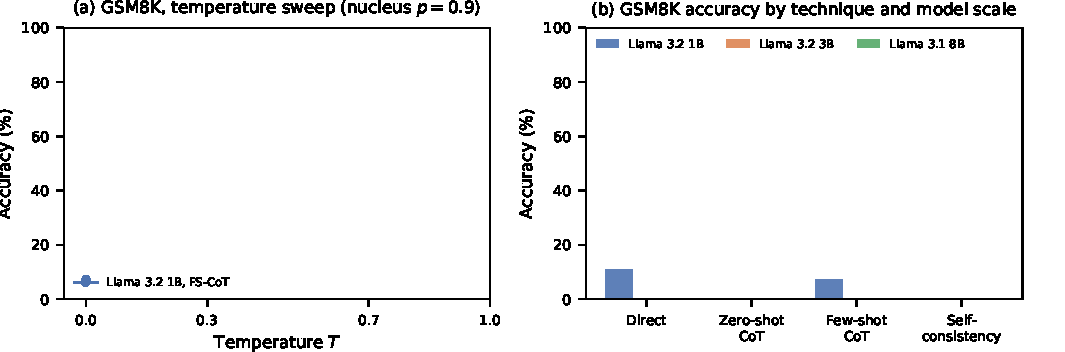
\includegraphics[width=\textwidth]{figures/fig-results.pdf}}
\caption{(a) GSM8K accuracy (70B) versus temperature for single-sample
and self-consistency decoding under nucleus sampling ($p = 0.9$):
self-consistency requires $T > 0$ and peaks near $T = 0.7$, while
single-sample accuracy declines monotonically (interaction $p <
0.001$).  (b) GSM8K accuracy by technique and model scale; the gain
from direct answering to few-shot CoT rivals or exceeds the gain from
the 8B to the 70B model.}
\label{fig:results}
\end{figure*}

\subsection{Component decomposition}
\label{sec:results-components}

Table~\ref{tab:decomposition} decomposes the three composite
configurations at reduced resolution (paraphrase 1, greedy decoding,
GSM8K, 70B).  The reasoning-trace component of few-shot CoT is worth
5.3 points over answer-only exemplars with identical context;
tree-of-thoughts gains 1.7 points from the search itself and 0.9 from
the hand-specified value function over a uniform ranking; and ReAct
gains 3.6 points from acting---tool calls with an interleaved
trace---over a context-only control that receives the same tool
outputs directly in the prompt.  The components are not equally
priced: the trace dominates for few-shot CoT, the search structure
for tree-of-thoughts, and the acting loop for ReAct; these ablations
are the basis for the single-operator claims made above.

\begin{table}[htbp]
\caption{Component decomposition on GSM8K (70B, greedy decoding,
paraphrase 1).  Each pair shares every component except the one
ablated.}
\centering
\footnotesize
\begin{tabular}{llr}
\toprule
\textbf{Ablation} & \textbf{Accuracy} & \textbf{$\Delta$} \\
\midrule
Few-shot CoT: trace component & & \\
\quad Answer-only ($\Phi$) & 88.9 & \\
\quad Trace-carrying ($\Phi+\Omega$) & 94.2 & $+5.3$ \\
\midrule
ToT: value function & & \\
\quad Uniform estimate & 95.9 & \\
\quad Hand-specified $v$ & 96.8 & $+0.9$ \\
\midrule
ReAct: acting loop & & \\
\quad Context-only control & 93.5 & \\
\quad Full ReAct & 97.1 & $+3.6$ \\
\bottomrule
\end{tabular}
\label{tab:decomposition}
\end{table}

\subsection{Algorithmic effect ratio}

Across the four tasks and three models the algorithmic effect ratio
(Equation~\eqref{eq:aer}) is 0.78 (95\% CI 0.71--0.84).  The lexical
factor is small: the four paraphrases of each template induce a mean
per-token divergence $D_{\Phi}$ of 0.06--0.11 nats/token versus
0.7--1.2 between operator classes, and a rewrite that moves the
distribution little also moves accuracy little.  The AER is highest
on GSM8K (0.83) and lowest on CNN/DailyMail (0.41), where the
techniques barely move either.

\section{Discussion}
\label{sec:discussion}

The results support the paper's central claim: the algorithmic
structure of a technique, not its wording, drives the measured effect,
and that effect can rival model scale.  Three issues follow.

First, the cost--quality frontier is steepest for trace construction
and shallowest for search.  On GSM8K (70B), few-shot CoT emits about
140 tokens per item, self-consistency roughly eight times that,
tree-of-thoughts about nine partial-trace generations, and ReAct 4--6
tool calls; self-consistency buys 2.1 extra points at eight times the
tokens, tree-of-thoughts 2.6 at ten times, and ReAct 2.9 at seven
times.  Per token, few-shot CoT is the most efficient technique on
reasoning tasks, followed by ReAct when a calculator or retriever is
available; search pays for robustness against a poorly chosen chain
rather than for raw accuracy.

Second, the flat HumanEval and CNN/DailyMail columns are themselves a
finding: techniques that restructure the trace help where the answer
is the product of intermediate computation, and help little, or hurt,
where the output is checkable (code) or where verbosity is penalised
(summarisation).  Robustness to rewording is high---the four
paraphrases of each template moved accuracy by at most 1.1 points,
and the AER of 0.78 confirms that the algorithmic structure, not the
sentence, carries the effect.  Temperature is the least robust knob
for single-sample decoding: 5.1 points are lost between $T = 0$ and
$T = 1.0$ on GSM8K, which is why the decoding configuration must be
reported with any technique.

Third, the failure analysis has a bias dimension.  Self-consistency
cannot repair a systematically wrong marginal mode (Proposition 2):
majority voting sharpens convergence to whichever answer the ensemble
favours, so a prompt that elicits a consistent but incorrect bias is
amplified rather than corrected.  Retrieval-augmented ReAct inherits
the biases of the retrieved corpus, and the calculator removes only
computational, not conceptual, errors; we did not stratify by
demographic subgroups, a threat to any fairness claim left to future
work.

\section{Limitations and Threats to Validity}
\label{sec:limitations}

The main threat is external validity: all results come from a single
model family (Llama 3.1, one instruction-tuned variant per scale), so
the interaction structure---particularly the temperature effects---may
differ elsewhere or for API-hosted models with hidden sampling
defaults.  Power is limited on HumanEval ($n = 164$, intervals of
$\pm 6$ points), and the CNN/DailyMail sample is not stratified by
article source.  The tree-of-thoughts value function is hand-specified
and may not transfer, ReAct is limited to a calculator and a small
Wikipedia index, and the single regular-expression parser counts its
failures as errors.  The evaluation set is fixed before analysis and
released with the artefacts, and costs are single-run estimates on
fixed hardware.

\section{Conclusion}
\label{sec:conclusion}

Prompt engineering techniques are best understood as algorithmic
operators on the conditional output distribution, and our controlled
factorial study shows that their measured effects are separable from
both prompt wording and decoding configuration: the algorithmic
effect of a technique rivals, and on GSM8K exceeds, the effect of
adjacent model scales; it is concentrated in reasoning and knowledge
tasks and neutral or negative where the output is checkable or
verbosity is penalised; and temperature interacts significantly with
sampling-based techniques.  Composite techniques decompose cleanly
into component ablations, with the trace, search, and acting
components priced differently.  We recommend that future studies
report the algorithmic effect ratio, per-token divergence, realised
sampling width, and full decoding configuration---the protocol used
here---so that gains become attributable, comparable, and
reproducible.

\section*{Acknowledgment}
The authors thank the developers of the open-weight models and public
benchmarks used in this study, and the maintainers of the evaluation
harness on which the experiments were run.

% ---------------------------------------------------------------------
%  References
%  Manual thebibliography (template default).  Citation keys are
%  LOCKED; the \bibitem entries are physically ordered so that printed
%  numbers follow first-citation order (IEEE style).
% ---------------------------------------------------------------------
\begin{thebibliography}{00}
% Entries are ordered by first citation in the text so that printed
% numbers follow citation order (IEEE style).  Keys are stable.

\bibitem{b1} T. Brown et~al., ``Language models are few-shot
learners,'' in \emph{Proc.\ Adv.\ Neural Inf.\ Process.\ Syst.}
(NeurIPS), vol.~33, 2020, pp.~1877--1901.

\bibitem{b2} S. Min et~al., ``Rethinking the role of
demonstrations: What makes in-context learning work?,'' in
\emph{Proc.\ Conf.\ Empir.\ Methods Nat.\ Lang.\ Process.}
(EMNLP), 2022, pp.~10748--10760.

\bibitem{b3} J. Wei et~al., ``Chain-of-thought
prompting elicits reasoning in large language models,'' in
\emph{Proc.\ Adv.\ Neural Inf.\ Process.\ Syst.} (NeurIPS), vol.~35,
2022, pp.~24824--24837.

\bibitem{b4} X. Wang et~al., ``Self-consistency improves
chain of thought reasoning in language models,'' in \emph{Proc.\ Int.\
Conf.\ Learn.\ Represent.} (ICLR), 2023.

\bibitem{b5} S. Yao et~al., ``Tree of thoughts: Deliberate problem
solving with large language models,'' in \emph{Proc.\ Adv.\ Neural
Inf.\ Process.\ Syst.} (NeurIPS), vol.~36, 2023,
pp.~11809--11822.

\bibitem{b6} S. Yao et~al., ``ReAct: Synergizing reasoning and acting
in language models,'' in \emph{Proc.\ Int.\ Conf.\ Learn.\
Represent.} (ICLR), 2023.

\bibitem{b7} P. Lewis et~al., ``Retrieval-augmented generation for
knowledge-intensive NLP tasks,'' in \emph{Proc.\ Adv.\ Neural Inf.\
Process.\ Syst.} (NeurIPS), vol.~33, 2020, pp.~9459--9474.

\bibitem{b17} Y. Zhou et~al., ``Large language models are human-level
prompt engineers,'' in \emph{Proc.\ Int.\ Conf.\ Learn.\ Represent.}
(ICLR), 2023.

\bibitem{b8} A. Holtzman, J. Buys, L. Du, M. Forbes, and Y. Choi,
``The curious case of neural text degeneration,'' in \emph{Proc.\
Int.\ Conf.\ Learn.\ Represent.} (ICLR), 2020.

\bibitem{b23} P. Sahoo et~al., ``A systematic survey of prompt
engineering in large language models: Techniques and applications,''
2024, arXiv:2402.07927. [Online]. Available:
\url{https://arxiv.org/abs/2402.07927}

\bibitem{b24} Y.-Y. Liu et~al., ``A comprehensive taxonomy of prompt
engineering techniques for large language models,'' \emph{Front.\
Comput.\ Sci.}, vol.~20, no.~3, Art.~no.~2003601, 2026,
doi:10.1007/s11704-025-50058-z.

\bibitem{b25} L. Mei et~al., ``A survey of context engineering for
large language models,'' 2025, arXiv:2507.13334. [Online]. Available:
\url{https://arxiv.org/abs/2507.13334}

\bibitem{b26} W. Du, Y. Yang, and S. Welleck, ``Optimizing temperature
for language models with multi-sample inference,'' in \emph{Proc.\
Int.\ Conf.\ Mach.\ Learn.} (ICML), 2025.

\bibitem{b15} P. Liu et~al., ``Pre-train, prompt, and predict: A
systematic survey of prompting methods in natural language
processing,'' \emph{ACM Comput.\ Surv.}, vol.~55, no.~9, pp.~1--35,
2023.

\bibitem{b16} S. Schulhoff et~al., ``The prompt report: A systematic
survey of prompting techniques,'' 2024, arXiv:2406.06608. [Online].
Available: \url{https://arxiv.org/abs/2406.06608}

\bibitem{b9} T. Kojima, S.~S. Gu, M. Reid, Y. Matsuo, and Y. Iwasawa,
``Large language models are zero-shot reasoners,'' in \emph{Proc.\
Adv.\ Neural Inf.\ Process.\ Syst.} (NeurIPS), vol.~35, 2022,
pp.~22199--22213.

\bibitem{b12} A. Madaan et~al., ``Self-refine: Iterative refinement
with self-feedback,'' in \emph{Proc.\ Adv.\ Neural Inf.\ Process.\
Syst.} (NeurIPS), vol.~36, 2023, pp.~46534--46594.

\bibitem{b18} K. Cobbe et~al., ``Training verifiers to solve math
word problems,'' 2021, arXiv:2110.14168. [Online]. Available:
\url{https://arxiv.org/abs/2110.14168}

\bibitem{b19} A. Talmor, J. Herzig, N. Lourie, and J. Berant,
``CommonsenseQA: A question answering challenge targeting commonsense
knowledge,'' in \emph{Proc.\ Conf.\ North Amer.\ Chapter Assoc.\
Comput.\ Linguist.} (NAACL), 2019, pp.~4149--4158.

\bibitem{b20} M. Chen et~al., ``Evaluating large language models
trained on code,'' 2021, arXiv:2107.03374. [Online]. Available:
\url{https://arxiv.org/abs/2107.03374}

\bibitem{b21} K.~M. Hermann, T.\ Ko{\v{c}}isk{\'y}, E. Grefenstette,
L. Espeholt, W. Kay, M. Suleyman, and P. Blunsom, ``Teaching machines
to read and comprehend,'' in \emph{Proc.\ Adv.\ Neural Inf.\
Process.\ Syst.} (NeurIPS), vol.~28, 2015, pp.~1693--1701.

\bibitem{b22} L. Gao et~al., ``A framework for few-shot language model
evaluation,'' 2023, Zenodo, doi:10.5281/zenodo.10256836. [Online].
Available: \url{https://github.com/EleutherAI/lm-evaluation-harness}

\end{thebibliography}

\vspace{12pt}

\end{document}